\documentclass[12pt,a4paper]{article}
%le préambule

\usepackage[T1]{fontenc}
\usepackage[francais]{babel}
\usepackage{url} % permet l'utilisation de la balise url pour les liens internet
\usepackage{graphicx} % permet l'utilisation des images

\title{Présentation du projet de dev web} % titre de l'article
\author{Anas Ben Abou / Simon Arnaud} % auteur de l'article
\date{16/05/2025} % date de l'article

%document principal
\begin{document}

\maketitle

\tableofcontents

\newpage

\section{Introduction :}
\subsection{Objectif du projet}
  Notre projet a eu pour but de réaliser un réseau social s'inspirant de X anciennement twitter, il nous a permis de mieux assimiler les connaissances apprises lors de nos cours et de comprendre réellement comment créer et gérer ce genre de plateforme. Nous nous sommes inspirés, mais nous avons également apporté notre propre vision à ce défi, en apportant une touche moins sombre et plus dynamique.\\
  
  %(\url{http://doc.ubuntu-fr.org/terminal})
  %\begin{center}
   %\includegraphics[width=350pt]{g12.png}
  %\end{center}
  
\subsection{Premières idées}
  Nos premières idées :
  \begin{itemize}
  \item Page très épurés au thème clair, doré.
  \item Lieu de partage -> modération importante (admin : droit de suppression de message)
  \item Possibilité de commenter, liker et partager le contenu.
  \end{itemize}
  

\subsection{Organisation}
  Pour ce projet, nous nous sommes organisés ...
  \begin{itemize}
  \item Répartition des rôles :
      \begin{itemize}
      \item Travail collectif. 
      \item Nous avons régulièrement discuté afin de correctement se répartir les tâches à chaque étape du développement.
      \end{itemize}
  \item Utilisation de github pour organiser nos avancées.
  \end{itemize}

\newpage

\section{Logique de notre programmation :}
\subsection{Base des pages et style}
  Afin d'avoir un site propre et fonctionnel, nous avons défini :
  \begin{itemize}
  \item deux headers différents pour gérer deux styles ;
  \item un footer permettant de se déplacer dans les différentes pages ;
  \item une fonction permettant de se connecter à notre base de données;
  \end{itemize}

\subsection{Les différentes pages}
  Voici la liste des pages que nous avons crées :
  \begin{center}
   \begin{tabular}{|c|c|} %tableau de 2 colonnes, dont le contenu est centré (c) et avec des bordures |
   \hline
   accueil & page d'accueil et de lecture des derniers posts \\
   \hline
   login,register & page de connexion et d'inscription \\
   \hline
   logout & page de déconnexion \\
   \hline
   profile & page du profile contenant les informations de l'utilisateur \\ & ainsi que ces publications \\
   \hline
   setting & page permettant de gérer son compte \\
   \hline
   message & page pour envoyer un message et afficher les messages reçus et envoyés \\
   \hline
   partage & page pour partager ses photos \\
   \hline
   followers & page pour voir le nombre d'abonnés  \\
   \hline
   following & page pour voir le nombre d'abonnements \\
   \hline
   \end{tabular}
  \end{center}
  
\section{Utilisation de notre base de donnée}
\subsection{Définition des tables}
  Afin de stocker efficacement les informations nécessaires au bon fonctionnement du site, nous avons définis plusieurs tables:
  
 \begin{itemize}
 \item users : id, nom, email, mot\_de\_passe, photo, bio, statut;
 \item posts : id, users\_id, contenu, date;
 \item likes : id, post\_id, user\_id;
 \item follows : id, follower\_id, following\_id;
 \item comments : id, post\_id, user\_id, contenu, date;
 \end{itemize}

\newpage

\subsection{Contraintes de stockage}

id : toujours définis pour toutes les tables;

Tables :
\begin{enumerate}
     


\item \textbf{user :}
  
  \begin{itemize}
    
  \item nom et email unique
  \item seul photo et bio peuvent ne pas avoir de valeur
  
  \end{itemize}

\item \textbf{posts :}
  
  \begin{itemize}
    
  \item clef étrangère : user\_id -> users.id
  
  \end{itemize}

\item \textbf{likes :}
  
  \begin{itemize}
    
  \item clef étrangère : post\_id -> posts.id
  \item clef étrangère : user\_id -> users.id
  
  \end{itemize}

\item \textbf{follows :}
  
  \begin{itemize}

  \item unique follower\_id et following\_id
  \item clef étrangère : follower\_id -> users.id
  \item clef étrangère : following\_id -> users.id
  
  \end{itemize}

\item \textbf{comments :}
  
  \begin{itemize}
    
  \item clef étrangère : post\_id -> posts.id
  \item clef étrangère : user\_id -> users.id
  
  \end{itemize}
    
\end{enumerate}

\section{Evolution}
\subsection{Personnel}

\begin{itemize}
    
  \item Grande évolution en PHP :
    \begin{itemize}
        
    \item Gestion de la base de donnée
    \item Gestion de la session
      
    \end{itemize}
    
  \item Renforcement de la compréhension de HTML, CSS et Javascript
    \begin{itemize}
        
    \item HTML : Utilisation des balises et compréhension de leurs différences.
    \item CSS : Organisation des différents éléments de façon propre et clair.
    \item Javascript : Rappel des différentes fonctionnalités.
      
    \end{itemize}
  
\end{itemize}

\newpage

\subsection{Projet}

Nous avons commencé par l'accueil afin de créer le premier style qui nous convenait et qui es resté un peu près le même.
Nous avons ensuite créer les pages d'inscription,connexion et déconnexion pour pouvoir effectuer la suite en prenant les valeurs stockés. Lors de la création de ses pages, nous avons commencé à utiliser la bdd en en définissant une première version bien moins complète.
Puis nous avons continuer avec la page du profile et du setting et avons enfin créer toutes les pages que nous avons actuellement. Nous avons ensuite fais évoluer chacune de nos pages à chaque fois que nous concevions de nouvelles fonctionnalités.

\section{Résultat final}
\subsection{Présentation du site}

\graphicspath{ {./} }

Voici la page d'accueil :
\begin{center}
  \includegraphics[scale=0.1]{image_5.eps}
\end{center}
Le corps de la page contient :
\begin{itemize}      

    \item une zone de texte pour publier un message
    \item La liste des publications les plus récentes.
      
\end{itemize}

\newpage

En haut de la page il y a deux boutons : un bouton pour le profile (à gauche) et un pour se déconnecter (à droite).
\begin{center}
  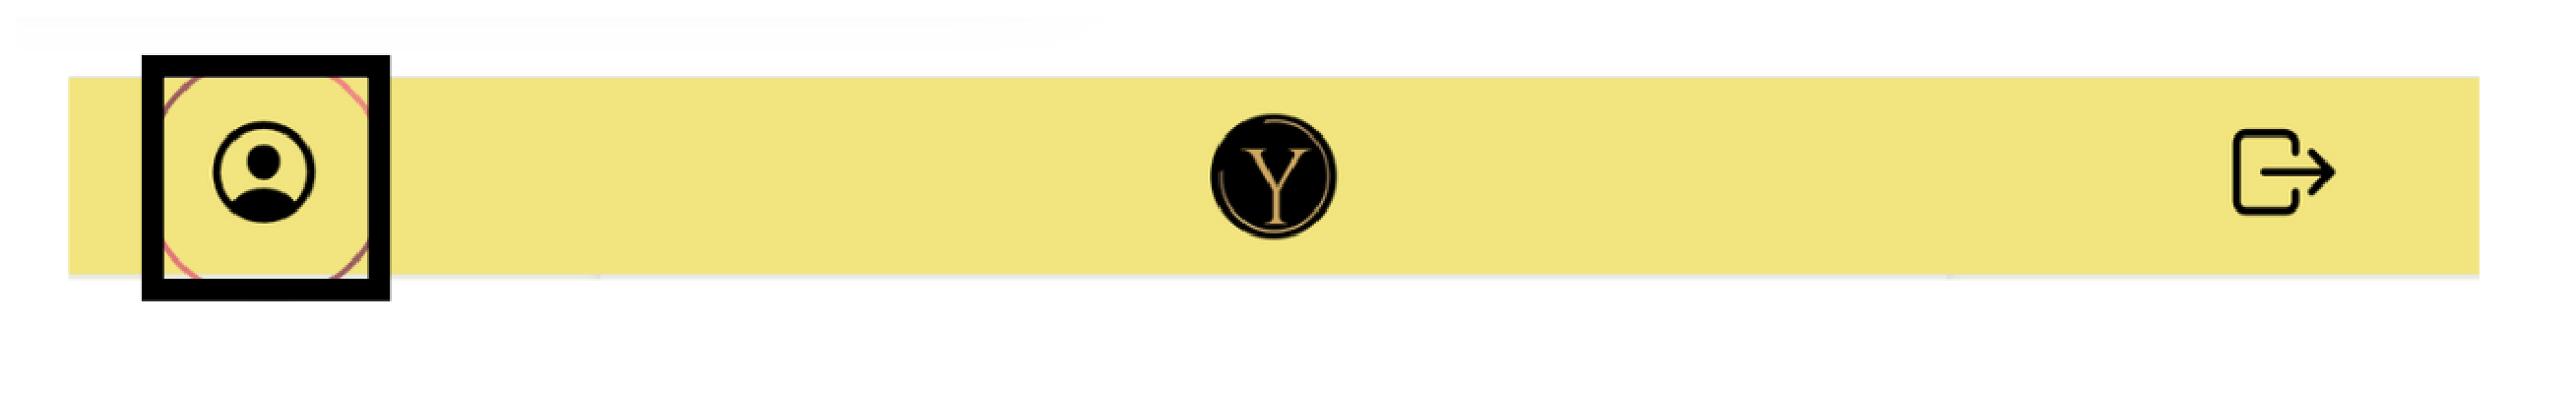
\includegraphics[scale=0.3]{image_1.eps}
\end{center}

En bas de la page il y a quatres boutons : ( de gauche à droite ) l'accueil, les paramètres, la messagerie, la page pour partager ses photos.
\begin{center}
  
\includegraphics[scale=0.2]{image_3.eps}
\end{center}

\subsection{Conclusion}

Pour conclure, ce projet nous a permit d'améliorer nos compétences en développement web.
Nous comptons poursuivre ce projet par delà cette soutenance afin d'arriver à un objectif finale qui serait de le publier en ligne.

\end{document}
